\section{Λογίσμικα που χρησιμοποιήθηκαν για την κατασκευή του server}

\subsection{Flask}

Για την ανάπτυξη του (διακομιστή ιστού) web server της IoT εφαρμογής,χρησιμοποιήσαμε την Flask.
Η Flash αποτελεί ένα ελαφρή framework της γλώσσας προγραμματισμού python 
για την δημιουργία web εφαρμογών,χρησιμοποιώντας το προτώκολλο Web Server Gateway Interface (WSGI) \cite{Flask}.
Η Flask αποτελεί μία από τις πιο δημοφιλές επιλογές framework για ανάπτυξη στον Ιστό,
μαζί με την FastAPI και την Django\cite{jetbrainsPopular}.

Το WSGI,όπως έχει οριστεί από την Python Enhancement Proposals 3333,αποτελεί ένα δημοφιλές προτώκολο της python για την διασύνδεσης 
διασύνδεσης μεταξύ web servers και web εφαρμογών \cite{PEP3333}.
Για την λειτουργία της,η Flask εξαρτάται από το WSGI toolkit και the Jinja template engine για την διμηουργία περιγραμμάτων (templates)
που διαμορφώνουν την μορφή της html στις σελίδων που επιστρέφει ο server στον (πελάτη) client.
Για server,χρησιμοποιήσαμε το Waitress έκδοσης 3.0.2 \cite{waitress},που είναι βασισμένο πλήρως στην python και στο πρότυπο WSGI.

Δεν θα περιγράψουμε ρητά πως αναπτύχθηκε η web εφαρμογή που διαχειρίζεται την http αιτήσεις,όπως κάναμε με τον μικροελεκτή. 
Η λειτουργία της web εφαρμογής θα φανεί σε σχέση με την αλλιλεπίδραση του server με τα άλλα προγράμματα που θα περιγράψουμε στην πορεία,
όπως και με την αλλιλεπίδραση του χρήστη με τον server.


\subsection{MongoDB}

Για την αποθήκευση και διαχείριση των δεδομένων που λαμβάνει ο server της εφαρμογής,χρησίιμοποιήσαμε την MongoDB Community Edition,
που αποτελεί την δωρεάν μορφή της MongoDB.
Η MongoDB αποτελεί μια βάση δεδομένων εγγράφων (documents database) που λειτουργεί σε πραγματικό χρόνο (Operational database).
Αποθηκεύει τα δεδομένα τις σε ευέλικτης δομής, JSON τύπου, documents(έγγραφα),το οποιο κάνει έυκολο την μοντελοποίηση δεδομένων με τον ίδιο τρόπο 
που τα χρησιμοποιεί και ο κώδικας των εφαρμογών που θα χρησιμοποιήσει τα δεδομένα.
Δεν επιβάλεται αυστήρη μορφή (schema) που πρέπει να έχουν τα δεδομένα, οπότε μπορούν να διαχειριστούμε μαζί documents με διαφορετική μορφή
και μπορούμε να αλλάξουμε την μορφή που έχουν τα document χωρίς πρόβλημα.

Ακόμα,Με την τεχνική Sharding δίνεται η δυνατότητα επέκτασης της βάσης δεδομένων σε πολλαπλά μηχανήματα,
δηλαδή οριζόντια επέκταση (Horizontal scaling),απελευθερώντνας μας από την ανάγκη του να προσθέσουμε παραπάνω
υπολογιστικούς πόρους σε ένα μηχάνημα στην περίπτωση που θέλαμε να επεκτήνουμε τις δυνατότητες της βάσης δεδομένων,
δηλαδή Vertical Scaling \cite{mongoDBoverview}.

Τα documents αποθηκεύονται με μορφή BSON,που είναι μια binary μορφή των json αντικειμένων, 
που υποστήριζει παραπάνω βασικούς τύπους δεδομένων από ότι τα json αντικείμενα.
Τα documents αποτελούνται από ζευγάρια πεδίων-τιμών, με τα πεδία να είναι πάντα τύπου String,δηλαδή απλώς κείμενο,
Οι τιμές να είναι οποιοδήποτε από τους βασικούς τύπους BSON, όπως είναι οι τύπου String,Boolean (λογικοί τύποι),Date(ημερομηνία) και άλλα,
αλλά και άλλα εμφολευμένο (nested) document,πίνακες και πίνακες από documnets.

Κάθε βάση δεδομένων (database),που ονομάζεται database στην Mongodb,χωρίζεται σε συλλογές (collection),
με τα collection να κατέχουν μέσα τους τα documents.
Τα collection ορίζονται περισσότερο για ομαδοποίηση documents με παρόμοια ταυτότητα.
Σε κάθε collection ενός database δίνεται ένα αμετάβλητο (immutable), χωρίς δυνατότητα τροποποίησης μετά aαπό την ανάθεση της τιμής,
μοναδικό αναγνωριστικό (Universally unique identifier,UUID) για να μπορέι να αναγνωριστεί μεταξύ των αντιγράφων του set στα διαφορετικά μηχανήματα
που μπορεί να βρίσκεται το collection.

Δεν επιβάλεται κάποιου είδος (schema) στα document.
Όμως,σε κάθε document ενός collection,όχι nested document,απαιτείται να έχει ένα πεδίο που ονομάζεται \texttt{\_id},
το οποίο έχει μονάδικη τιμή για το συγκεκριμένο collection, η οποία δεν επαναλαμβάνεται η τιμή αυτή για πεδίο \texttt{\_id} κάπου αλλού στο collection
To \texttt{\_id} είανι το κύριο κλειδή του document,δηλαδή το αναγνωριστικό του για να ξεχωρίζει σε σχέση με τα υπόλοιπα documents.
Εάν δεν δωθεί πεδίο με όνομα \texttt{\_id}, τότε η ίδια η mongoDB το προσθέτει στο document,
δημιουργώντας μια τιμή τύπου ObjectId.

Οι δύο κύριοι λόγοι για τους οποίους επιλέχθηκε η MongoDB είναι ότι κάνει πολύ εύκολη την αποθήκευση των
δεδομένων που έρχονται από τις συσκευές μας και κρατάει ανέπαφη την json μορφή των δεδομένων.
Η κάθε δειγματοληψία,μαζί με τις έξτρα πληροφορίες που προστέθηκαν από τους μικροελεκτές,
το id της συσκευής,δηλαδή του μικροελεκτή μαζί με τον αισθητήρα,την χρονική στιγμή που συλλέχθηκε η δειγματοληψία 
και το όνομα του αισθητήρα που έκανε την δειγματοληψία,αποτελούν αυτόνομα json αντικείμενα και δεν χρειάζονται να γνωρίζουν πληροφορίες μεταξύ τους.


Για την εφαρμογή μας,χρησιμοποιήθηκαν δύο collection.
Το πρώτο collection, που είναι και το πιο μεγάλο σε όγκο δεδομένων,περιέχει τα δεδομένα που έχουν στείλει οι μικροελεκτές στον server.
Κάθε ξεχωριστό document είναι μία δειγματοληψία που έχει πραγματοποιηθεί.
Η μορφή των documents βασίζονται στην μορφή των δεδομένων όπως τα έστειλε ο μικροελεκτής στο server.
Τα documents από αισθητήρες με το ίδιο όνομα έχουν πάντα την ίδια μορφή δεδομένων

Το δεύτερο collection περιέχει τα δεδομένα που έχουμε πάρει από τον χρήστη,μέσω του client-sided (πλευρά του πελάτη) κομματιού της web εφαρμογής που έχουμε δημιουργήσει.
Είναι δεδομένα που ο χρήστης δηλώνει ρητά στο server,που σκοπό έχουν την συμπλήρωση στοιχείων που θα χρησιμοποιήσουμε για την μετέπειτα επεξεργασία των μετρήσεων που συλέχθηκαν στα πειράματα.
Το  μας υποδικνύει τι κατηγορία δεδομένων είναι,αν και μπορεί να υπάρχουν διαφορετικές υποκατηγορίες με βάση την κατηγορία.

Η ανάγκη για διαφορετικές κατηγορίες προέκυψε γιατί είχαμε υλοποιήσει την δυνατότητα για τον χρήστη να εισάγει θερμοκρασία και υγρασία δωματίου,με γνώση που υπήρχε από όργανο εκτός των αισθητήρων.
Οι δύο σκοποί της λειτουργίας αυτής είναι η αποστολή των δεδομένων αυτών σε αισθητήρες που το χρειάζονται για καλύτερο υπολογισμο της ποιότητας του άερα,όπως ήταν ο CCS811,και η συμπερίληψη των 
περιβαλλοντικών συνθήκων στην μετέπειτα ανάλυση και υλοποίηση των μηχανικών μοντέλων,χωρίς να βασιζόμαστε μόνο στις τιμές του αισθητήρα θερμοκρασία και υγραφίας του ΒΜΕ680.

Δεν χρησιμοποήθηκε η συγκεκριμένη λειτουργία στα πειράματα,γιατί ο CCS811 που το χρησιμοποιήσε σαν πληροφορίας,σταματήσαμε να το χρησιμοποιούμε πριν την έναρξη των πειραμάτων.Kαι o bme680 
δεν χρησιμοποιεί εξωτερικές μετρήσεις,καθώς έχει τους δικούς του αισθητήρα.
Και δεν εντάξαμε τις περιβαλλοντικές συνθήκες,καθώς η BSEC συμπεριλαμβάνει είδη την υγρασία και θερμοκρασία στα μοντέλα που υπολογίζουν την ποιότητα του αέρα.
Μην ξέροντας πως λειτουργούν τα εσωτερικά μοντέλα της BSEC,και αφού δεν προσεγγίσαμε την εύρεση της πηγής ρύπου με κάποιο μοντέλο που περιλαμβάνει υγρασία και θερμοκρασία,
δεν έχει νόημα να απαιτούμε από τον χρήστη να συλλέγει την θερμοκρασία και υγρασία,είδικα στην συχνότητα που απαιτεί τέτοια ανάλυση.
Το όργανο που χρησιμοποιήθηκε για την μέτρηση ποιότητας και υγρασίας δεν είχε κάποιο τρόπο αποστολής δεδομένων στον υπολογιστή.
Παρόλα αυτά,έχει παραμείνει η συγκεκριμένη λειοτουργία,σε περίπτωση που μελλοντικα χρειάζεται η γνώση της θερμοκρασίας και υγρασίας από εξωτερικό μετρήτη για τους δύο παραπάνω λόγους που αναφέραμε.

Οπότε η βασική κατηγορία δεδομένων για το collection σχετικά με τον χρήστη είναι αυτά που στο πεδίο \texttt{UserInputCategory}, έχουν τιμή \texttt{ExperimentState}.
Στα πειράματα μας,τα δεδομένα αυτά χωρίζονται σε τρεις υποκατηγορίες,με βάση την τιμή που έχουν στο πεδίο \texttt{ExperimentState}.
Οι τρεις υποκατηγορίες είναι οι καταστάσεις του πειράματας \texttt{StartingExperiment},\texttt{InsertingSourcePollutant} και \texttt{RemovingSourcePollutant}.
Η πρώτη και η τρίτη υποκατηγορία έχουν σαν βασικά και μόνο πεδίο που κράταμε την χρονική στιγμή που δηλώνονται από τον χρήστη.
Η κατάσταση \texttt{InsertingSourcePollutant} εκτός από την χρονική στιγμή,έχει και αλλές λεπτομέρειες που δίνουν στοιχεία για την πηγή του ρύπου και τις συνθήκες του πειράματος.
Οι λεπτομέρειες θα περιγραφτούν όταν μιλήσουμε για την διαδικασία πειραμάτων.


 \begin{figure}[!htbp]
     \centering
    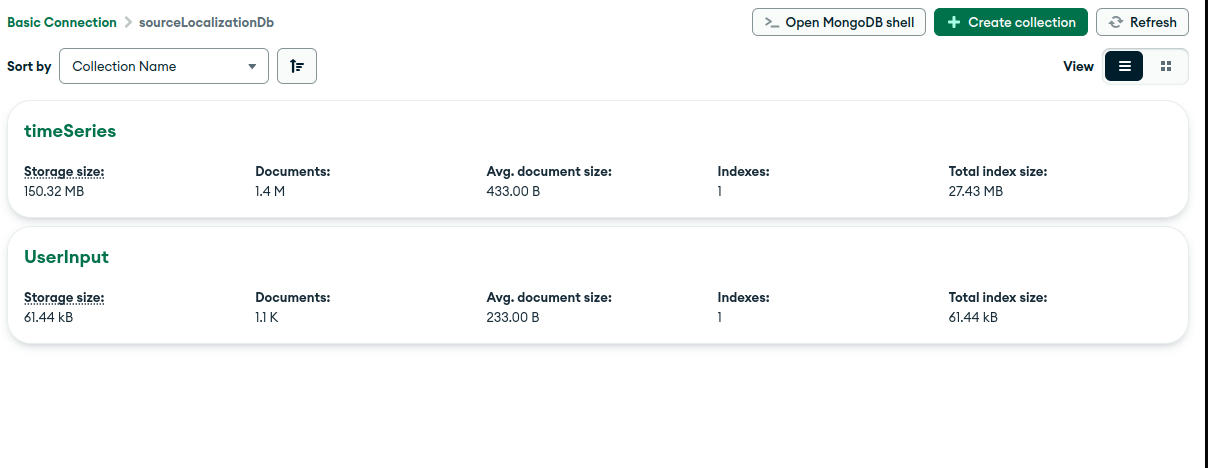
\includegraphics[width=0.8\textwidth]{εικόνες/εικόνες σχετικά με τον server/mongodbCollections.png}
     \caption{Οι συλλογές της βάσεις δεδομένων τις εφαρμογής}
     \label{fig:mongoDBcollection}
 \end{figure}

\begin{figure}[!htbp]
    \centering
    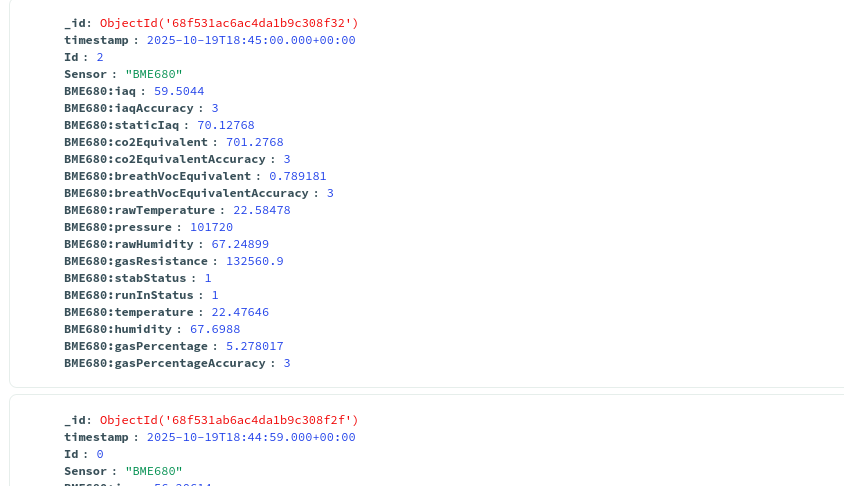
\includegraphics[width=0.8\textwidth]{εικόνες/εικόνες σχετικά με τον server/time series document.png}
    \caption{Μορφή documents στο collection που εμπεριέχει τα δεδομένα του χρήστη}
    \label{fig:userTimeSeries}
\end{figure}


\begin{figure}[!htbp]
    \centering
    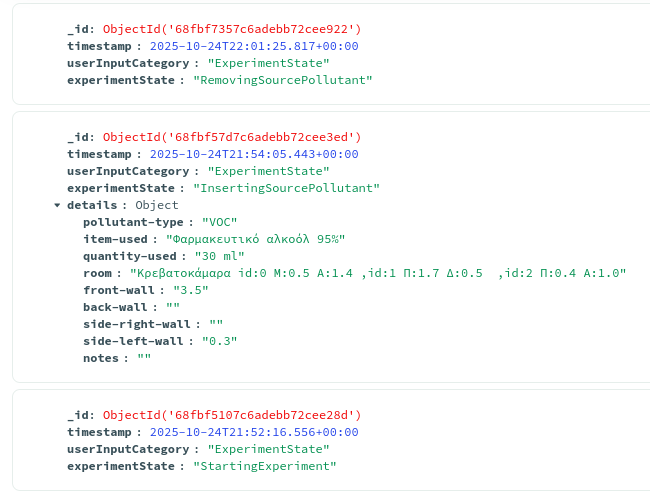
\includegraphics[width=0.8\textwidth]{εικόνες/εικόνες σχετικά με τον server/userDatadocumentCropped.png}
    \caption{Μορφή documents στο collection που εμπεριέχει τα δεδομένα του χρήστη}
    \label{fig:userDocument}
\end{figure}

\FloatBarrier 


\subsection{Grafana:Για οπτικοποίηση}

Χρησιμοποιήσαμε την Grafana Open Source Software (OSS) για να οπτικοποιήσουμε τις μετρήσεις των αισθητήρων σε ζωντανό χρόνο.
Το Grafana είναι λογισμικό ανοιχτού κώδικα για την οπτικοποίηση και την ανάλυση δεδομένων.
Επιτρέπει την αναζήτηση(queries),οπτικοποιήση και εξερεύνηση μετρικών δεδομένων,αρχείων καταγραφής (logs) και τα traces,
ανεξάρτητα από το πού είναι αποθηκευμένα.
Επίσης,παρέχει εργαλεία για την μετατροπή δεδομένων χρονοσειρών TSDB σε κατανοητά γραφήματα και οπτικοποιήσεις \cite{grafana}.


Οι χρονοσειρές ορίζονται εώς ταξινομημένες ακολουθία τιμών μιας μεταβλητής σε ισαπέχοντα χρονικά διαστήματoς \cite{timeSeriesDefinition}.
Οι μετρήσεις των αισθητήρων αποτελούν ένα είδος χρονοσειρας,αν και πρέπει να διαχωρίσουμε τις διαφορετικούς εξόδους των αισθητήρων
σε διαφορετικές απεικονίσεις των χρονοσειρών.Όλοι οι αισθητήρες με το ίδιο όνομα βρίσκονται στο ίδιο dashboard για μια συγκεκριμένη μετρική.
Έχουμε χωρίσει τις συγκεκριμένες εξώδεις που φαίνονται στο \ref{fig:grafana},αλλά μπορεί να προστεθεί οποιαήποτε από τις εξόδους που έχουμε από τον κάθε αισθητήρα.

Το βασικό κομμάτι της Grafana είναι οι ψηφιακές πίνακες ελέγχου (Dashboard)

 \begin{figure}[!htbp]
     \centering
     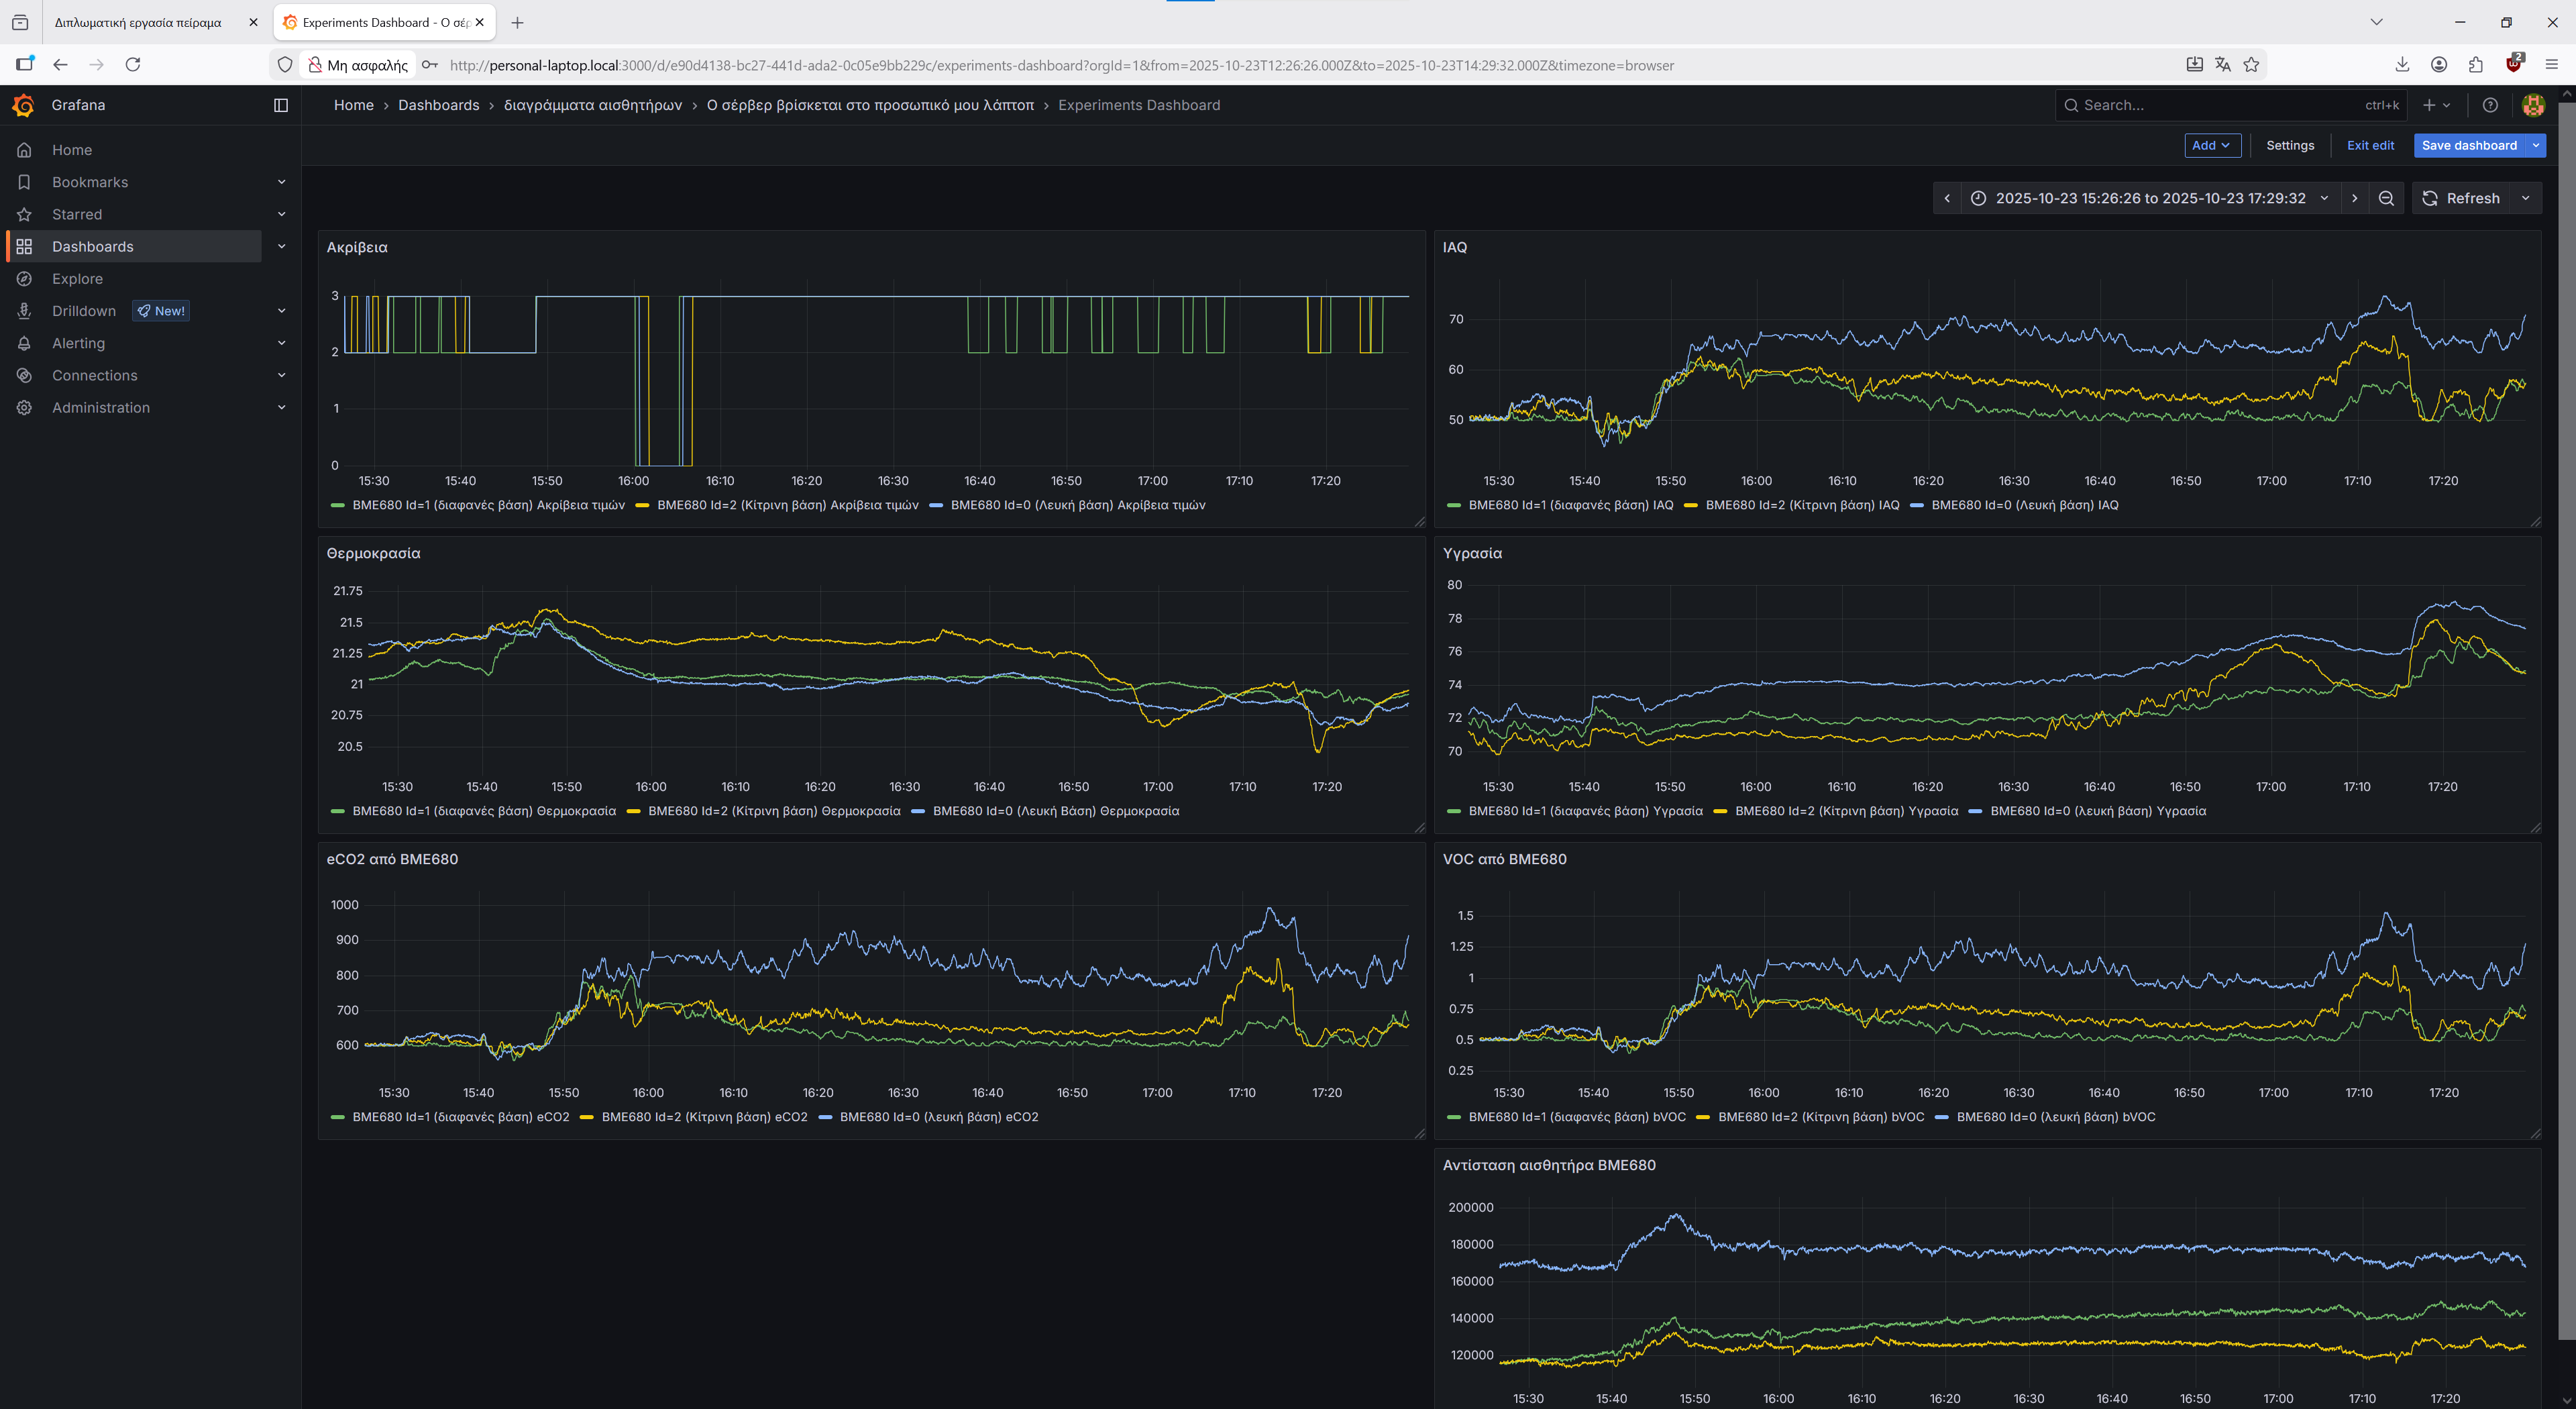
\includegraphics[width=0.8\textwidth]{εικόνες/εικόνες σχετικά με τον server/grafana dashboard.png}
     \caption{Grafana dashboard κατά την διάρκεια των πειραμάτων}
     \label{fig:grafana}
 \end{figure}

\FloatBarrier 
